La topologia di rete di Blue Agent è suddivisa logicamente in due reti:

\begin{itemize}
\tightlist
\item
  \textbf{Una rete di produzione per ogni team}, dove la rete
  \(\text{production-}k\) identifica gli oggetti di rete ed i container
  necessari al team \(k\).
\item
  \textbf{Al più una rete di verifica per ogni team}, dove la rete
  \(\text{verify-}k\) identifica gli oggetti di rete ed i container
  duplicati utilizzati per la verifica richiesta dal team \(k\).
\end{itemize}

Lo schema di indirizzamento prevede una netta separazione tra lo spazio
di gioco del team \(k\), la rete WireGuard e la rete di Incus:

\begin{itemize}
\tightlist
\item
  \passthrough{\lstinline!10.k.0.0/24!}: è la sottorete WireGuard per i
  membri del team \(k\).
\item
  \passthrough{\lstinline!10.k.1.0/24!}: è la sottorete LAN per i
  container di produzione e per i cloni di verifica.
\item
  \passthrough{\lstinline!172.16.0.0/24!}: è la sottorete gestita da
  \(\text{incusbr0}\) per fornire la connettività esterna e le reti OVN
  tramite NAT.
\end{itemize}

\section{\texorpdfstring{Rete
\(\text{production-}k\)}{Rete \textbackslash text\{production-\}k}}\label{rete-textproduction-k}

La rete \(\text{production-}k\) (Figura \ref{fig:production-network}) è
progettata per offrire un ambiente isolato e raggiungibile
esclusivamente dai membri autorizzati del team. È costituita dai
seguenti dispositivi di rete:

\begin{itemize}
\tightlist
\item
  \(\text{wg-}k\): dispositivo L3 gestito da WireGuard, fa da
  terminazione per il tunnel del team \(k\)-esimo. Ha come IP gateway:
  \passthrough{\lstinline!10.k.0.1/24!}
\item
  \(\text{br-team-}k\): dispositivo L2 gestito dal kernel Linux. Ha come
  IP gateway: \passthrough{\lstinline!10.k.1.1/24!}
\item
  \(\text{eth0}\): le interfacce di rete \(\text{eth0}\) dei container
  che vengono collegate a \(\text{br-team-}k\).
\end{itemize}

\(\text{wg-}k\) serve per fornire ai membri del team \(k\) l'endpoint
per la connessione tramite VPN, in questo modo i membri del team saranno
connessi direttamente alla rete \(\text{production-}k\). Ogni membro ha
la sua configurazione WireGuard associata al suo peer impostato
sull'interfaccia \(\text{wg-}k\). Aggiungere un peer all'interfaccia
WireGuard significa permettere ad un client con una certa chiave
pubblica di collegarsi con un certo indirizzo ip (\textbf{cryptokey
routing}), e quindi assegnare ad ogni membro del team \(k\) un indirizzo
nella sottorete \passthrough{\lstinline!10.k.0.0/24!}.

L'interfaccia \(\text{br-team-}k\) permette di creare una rete LAN per i
container del team \(k\), a cui questi si collegano.

Questo collegamento avviene tramite l'utilizzo di una
\passthrough{\lstinline!veth pair!} (Virtual Ethernet) per container:
un'estremità è collegata a \(\text{br-team-}k\), l'altra all'interfaccia
del container \passthrough{\lstinline!eth0!}. Questa architettura
comporta la creazione di un numero di \passthrough{\lstinline!veth!}
pair lineare al numero di container attivi.

\begin{quote}
\passthrough{\lstinline!veth!}: È utile per collegare interfacce che
risiedono per esempio su differenti Network Namespace (ossia il modo in
cui sono implementati i container). Utilizzano poca CPU e poca memoria,
dato che l'implementazione è efficiente e risiede direttamente nel
kernel. Dunque per centinaia di \passthrough{\lstinline!veth!} non si ha
un degrado evidente delle prestazioni. \footnote{\label{fn:ref_16}Linux manual page,
  veth(4) - Virtual Ethernet Device:
  https://man7.org/linux/man-pages/man4/veth.4.html}
\end{quote}

Tramite regole di forwarding del kernel e di firewall via
\passthrough{\lstinline!nftables!}, il traffico dell'interfaccia
\(\text{wg-}k\) viene autorizzato verso \(\text{br-team-}k\) e
viceversa. Questa regola viene applicata aggiungendo dentro al set
\passthrough{\lstinline!team\_links!} (una struttura dati all'interno
del kernel gestita da nftables) la coppia di interfacce interessate.


\begin{figure}[!htbp]
  \centering
  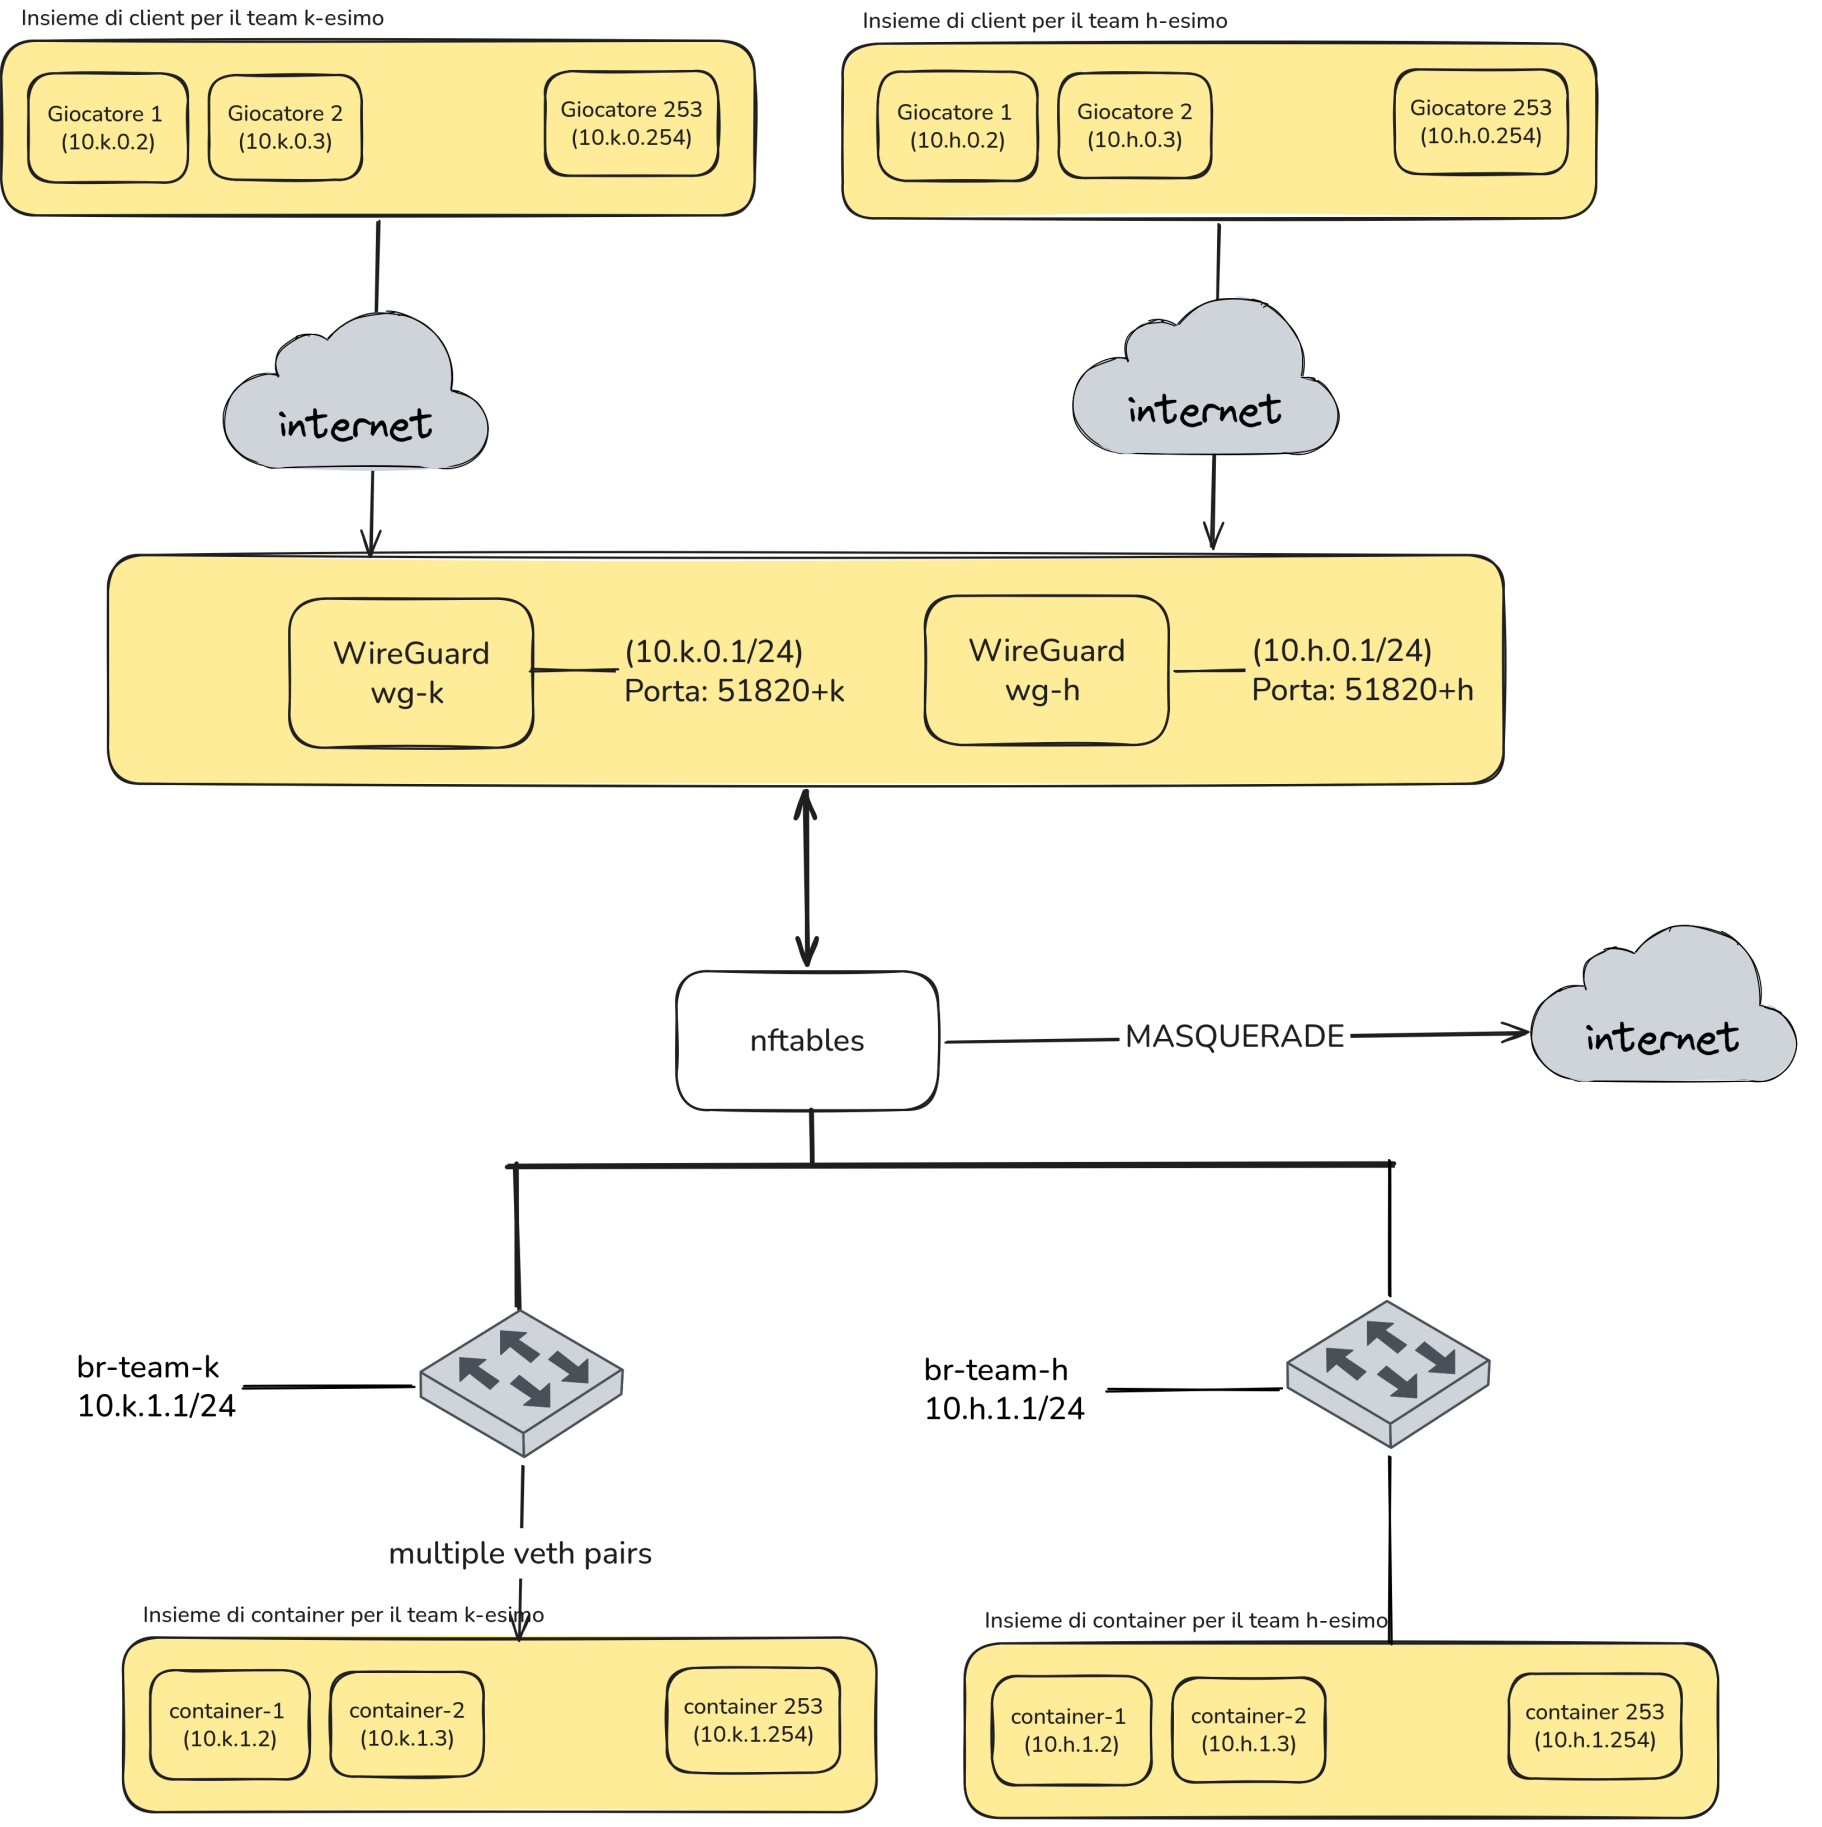
\includegraphics[width=0.60\linewidth,height=0.32\textheight,keepaspectratio]{src/images/production-network.png}
  \caption[Topologia della rete di produzione per il team k]{Topologia della rete di produzione (\text{production-}k) per il team $k$}
  \label{fig:production-network}
\end{figure}


\begin{center}\rule{0.5\linewidth}{0.5pt}\end{center}

\section{\texorpdfstring{Rete
\(\text{verify-}k\)}{Rete \textbackslash text\{verify-\}k}}\label{rete-textverify-k}

La rete \(\text{verify-}k\) (Figura \ref{fig:verify-network}) è
costituita dai seguenti componenti:

\begin{itemize}
\tightlist
\item
  \(\text{verify-}k\): rete virtuale logica gestita via SDN tramite OVN
  e orchestrata da Incus \footnote{\label{fn:ref_17}Documentazione ufficiale Incus, OVN
    network driver:
    https://linuxcontainers.org/incus/docs/main/reference/network\_ovn/}.
  Non costituisce una singola interfaccia di rete convenzionale del
  kernel, ma una topologia virtuale isolata composta da uno switch e un
  router con gateway: \passthrough{\lstinline!10.k.1.1/24!}.
\item
  \(\text{incusbr0}\): bridge di rete di Incus con gateway
  \passthrough{\lstinline!172.16.0.1/24!}. Svolge il ruolo di
  interfaccia per l'instradamento verso l'esterno della rete OVN.
\item
  \(\text{eth0}\): sono le interfacce di rete dei container clonati
  (\passthrough{\lstinline!10.k.1.x!}) che vengono collegate a
  \(\text{verify-}k\).
\end{itemize}

\begin{quote}
Incus è in grado di gestire da solo il collegamento tra
\(\text{incusbr0}\) e \(\text{verify-}k\). Questo semplifica di molto la
gestione delle interfacce di verifica per BlueAgent.
\end{quote}

Le interfacce dei container e la rete \(\text{verify-}k\) sono gestite
dalla SDN (\emph{Software Defined Network}). \(\text{verify-}k\) è
implementata da:

\begin{enumerate}
\def\labelenumi{\arabic{enumi}.}
\tightlist
\item
  un \textbf{Logical Switch} (denominato internamente da Incus nel DB di
  OVN come \passthrough{\lstinline!incus-net<ID>-ls-int!} \footref{fn:ref_17}):
  rappresenta la LAN su cui si agganciano le interfacce virtuali dei
  container di verifica.
\item
  un \textbf{Logical Router} (denominato
  \passthrough{\lstinline!incus-net<ID>-lr!} \footref{fn:ref_17}):
  agisce come gateway (\passthrough{\lstinline!10.k.1.1/24!}),
  permettendo ai container clonati di preservare l'identica
  configurazione IP rispetto alla produzione.
\end{enumerate}

\begin{quote}
\textbf{Tunneling Geneve e considerazioni sull'MTU:} OVN impiega il
protocollo di tunneling \textbf{Geneve} (\emph{Generic Network
Virtualization Encapsulation}) \footnote{\label{fn:ref_18}Documentazione architetturale
  OVN e Geneve: https://docs.ovn.org/en/latest/topics/geneve.html} per
spostare i pacchetti tra più nodi della rete.
\end{quote}

L'incapsulamento Geneve introduce tuttavia un overhead di intestazione
variabile (fino a 58 byte), riducendo l'MTU effettiva della rete a
\(1442\) byte (rispetto ai 1500 byte dello standard Ethernet). Se
pacchetti di dimensione eccedente hanno il flag \emph{Don't Fragment}
(DF) abilitato, rischiano di essere scartati generando un fenomeno di
\emph{Path MTU Blackhole}.

Bisogna notare che il tunnel Geneve non viene mai utilizzato, poiché i
container di verifica risiedono tutti all'interno dello stesso nodo.
Tuttavia Incus limita di default l'MTU delle interfacce di rete dei
container a 1442 byte per precauzione; per risolvere il problema è
possibile forzare l'MTU a 1500.

L'uso di una SDN garantisce l'assenza di conflitti di routing grazie a
una netta separazione tra \textbf{spazio utente} e \textbf{spazio
kernel} \footnote{\label{fn:ref_19}Documentazione Open vSwitch, architettura Datapath
  Kernel vs Userspace:
  https://docs.openvswitch.org/en/latest/intro/what-is-ovs/}:

\begin{itemize}
\tightlist
\item
  \textbf{Spazio Utente (Control Plane):} i demoni di controllo di OVN
  (\passthrough{\lstinline!ovn-northd!} e l'agente locale
  \passthrough{\lstinline!ovn-controller!}) elaborano la topologia
  logica e la traducono in flussi OpenFlow concreti per Open vSwitch
  (\passthrough{\lstinline!ovs-vswitchd!}). Il router OVN esiste
  puramente a livello logico.
\item
  \textbf{Spazio Kernel (Data Plane):} il demone
  \passthrough{\lstinline!ovs-vswitchd!} riceve i flussi OpenFlow e
  programma il modulo kernel \passthrough{\lstinline!openvswitch.ko!},
  dove viene applicato l'inoltro dei frame ad alte prestazioni.
\end{itemize}

Il collegamento tra i container e la rete OVN sfrutta sempre una coppia
\passthrough{\lstinline!veth!}: un'estremità risiede all'interno del
container e si attacca ad \passthrough{\lstinline!eth0!}, mentre l'altra
estremità sull'host viene agganciata direttamente al bridge di Open
vSwitch.

\begin{quote}
\passthrough{\lstinline!SDN (Software Defined Networking)!}: Paradigma
architetturale che separa il \textbf{piano di controllo} dal
\textbf{piano dei dati}, consentendo di gestire e programmare
l'infrastruttura di rete interamente via software.
\end{quote}

\begin{quote}
\passthrough{\lstinline!OpenFlow!}: Protocollo standard che permette al
controller SDN di comunicare con lo switch e programmare le regole di
matching e le azioni direttamente all'interno delle pipeline di Open
vSwitch.
\end{quote}

\begin{quote}
\passthrough{\lstinline!OVN (Open Virtual Network)!}: Sistema SDN che
opera come Control Plane per Open vSwitch. Traduce topologie logiche
(Logical Switch, Logical Router, NAT e ACL) tramite
\passthrough{\lstinline!ovn-northd!} e
\passthrough{\lstinline!ovn-controller!} in flussi OpenFlow distribuiti,
istruendo Open vSwitch su come instradare il traffico senza creare
molteplici interfacce o bridge dedicati nel kernel host. È costituito da
due database: \textbf{OVN Northbound}: memorizza la dichiarazione delle
reti logiche da creare e le proprietà che devono rispettare. \textbf{OVN
Southbound:} memorizza le tabelle di flussi logici compilate da
\passthrough{\lstinline!ovn-northd!}, che
\passthrough{\lstinline!ovn-controller!} traduce in regole OpenFlow
concrete per il piano dei dati.
\end{quote}

La comunicazione verso l'esterno avviene collegando il Logical Router
OVN al bridge parent \(\text{incusbr0}\), da cui ottiene un indirizzo IP
da utilizzare. L'accesso a Internet per i container di verifica sfrutta
un meccanismo di NAT a due stadi:

\begin{itemize}
\tightlist
\item
  \textbf{Primo Stadio (SNAT in OVN)}: quando un container di verifica
  (\passthrough{\lstinline!10.k.1.x!}) invia traffico all'esterno, il
  Logical Router riscrive l'indirizzo sorgente sostituendolo con l'IP
  assegnatogli da \passthrough{\lstinline!incusbr0!} (nella sottorete
  \passthrough{\lstinline!172.16.0.0/24!}). Se non fosse applicato, i
  pacchetti in uscita manterrebbero l'indirizzo sorgente
  \passthrough{\lstinline!10.k.1.x!}, i quali sono attestati sulle
  interfacce di rete dei container nella rete di produzione.
\item
  \textbf{Secondo Stadio (SNAT su \passthrough{\lstinline!incusbr0!})}:
  una volta raggiunto \passthrough{\lstinline!incusbr0!}, il
  sottosistema Netfilter, tramite regole
  \passthrough{\lstinline!nftables!}, applica la regola di
  \textbf{masquerade} verso l'interfaccia fisica per uscire su Internet.
  Viene sostituito l'indirizzo di \passthrough{\lstinline!incusbr0!} con
  l'indirizzo pubblico dell'host che esegue BlueAgent.
\end{itemize}

\begin{longtable}[]{@{}
  >{\raggedright\arraybackslash}p{(\linewidth - 6\tabcolsep) * \real{0.2889}}
  >{\raggedright\arraybackslash}p{(\linewidth - 6\tabcolsep) * \real{0.2889}}
  >{\raggedright\arraybackslash}p{(\linewidth - 6\tabcolsep) * \real{0.2593}}
  >{\raggedright\arraybackslash}p{(\linewidth - 6\tabcolsep) * \real{0.1630}}@{}}
\toprule\noalign{}
\begin{minipage}[b]{\linewidth}\raggedright
Tratta del Pacchetto
\end{minipage} & \begin{minipage}[b]{\linewidth}\raggedright
Indirizzo Sorgente (\(IP_{src}\))
\end{minipage} & \begin{minipage}[b]{\linewidth}\raggedright
Indirizzo Destinazione (\(IP_{dst}\))
\end{minipage} & \begin{minipage}[b]{\linewidth}\raggedright
Responsabile
\end{minipage} \\
\midrule\noalign{}
\endhead
\bottomrule\noalign{}
\endlastfoot
Dal Container ad \passthrough{\lstinline!incusbr0!} &
\passthrough{\lstinline!10.k.1.x!} \emph{(IP duplicato)} & \(IP_{ext}\)
\emph{(Internet)} & Container di verifica \\
Da \passthrough{\lstinline!incusbr0!} all'interfaccia dell'host &
\passthrough{\lstinline!172.16.0.x!} \emph{(IP transito univoco)} &
\(IP_{ext}\) \emph{(Internet)} & Incus \\
Dall'host verso l'esterno & IP dell'interfaccia pubblica dell'host. &
\(IP_{ext}\) \emph{(Internet)} & \passthrough{\lstinline!nftables!} /
Netfilter \\
\end{longtable}

Il NAT a due stadi è necessario per evitare collisioni di routing
sull'Host: il primo stadio ``nasconde'' gli indirizzi duplicati
\passthrough{\lstinline!10.k.1.x!} traducendoli in un IP su
\passthrough{\lstinline!172.16.0.0/24!}, mentre il secondo stadio
permette la navigazione esterna condividendo l'IP dell'host.

\begin{quote}
\passthrough{\lstinline!NAT (Network Address Translation)!}: Meccanismo
di rete che modifica le informazioni di intestazione IP (e opzionalmente
le porte di livello 4) dei pacchetti in fase di routing. \footnote{\label{fn:ref_20}Documentazione
  Netfilter, Network Address Translation (NAT):
  https://wiki.nftables.org/wiki-nftables/index.php/Performing\_Network\_Address\_Translation\_(NAT)}.
\end{quote}

\begin{quote}
\passthrough{\lstinline!SNAT (Source NAT)!}: Variante del NAT applicata
al traffico uscente (\textbf{egress}, fase di postrouting). Modifica
l'indirizzo IP sorgente del pacchetto con un indirizzo pubblico o
instradabile dalla rete esterna.
\end{quote}

\begin{quote}
\passthrough{\lstinline!Masquerading!}: Variante dinamica di
\passthrough{\lstinline!SNAT!}. Si ha quando l'indirizzo sorgente viene
mappato dinamicamente sull'IP dell'interfaccia di uscita dell'host.
\end{quote}


\begin{figure}[!htbp]
  \centering
  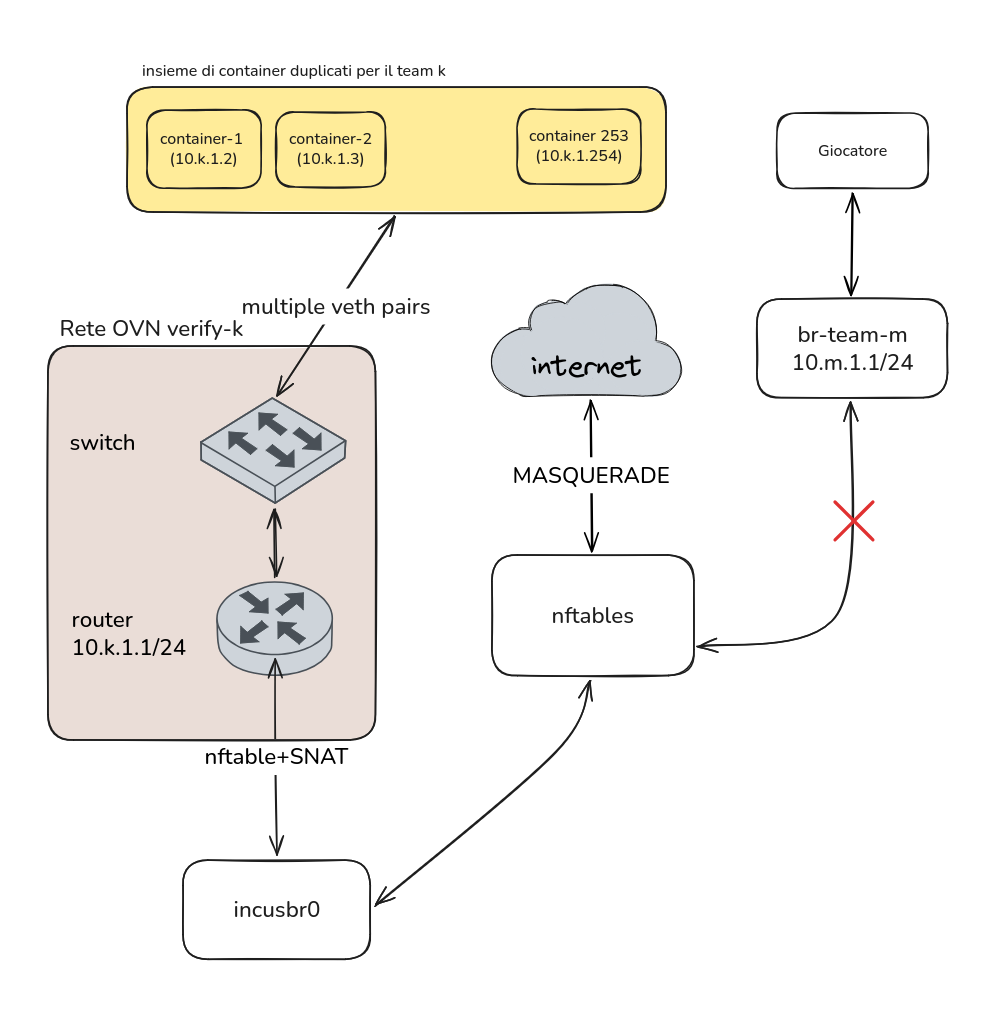
\includegraphics[width=0.60\linewidth,height=0.32\textheight,keepaspectratio]{src/images/verify-network.png}
  \caption[Topologia della rete di verifica sandbox per il team k]{Topologia della rete di verifica sandbox (\text{verify-}k) orchestrata con OVN}
  \label{fig:verify-network}
\end{figure}

